\documentclass{astroedu-lab}

\begin{document}

\pagestyle{plain}

\begin{problem}{\huge Радиотехническая работа 25\\\\Лестничные фильтры\\\\Выполнил Жданов Елисей Б01-205}

\section{Оборудование:}

ПО Micro-Cap 10.0.7.0

\section{Задание}

\subsection{Ознакомительные шаги}

Задание выполняется в Micro-Cap

\subsection{Трехполюсные лестничные фильтры}

\begin{enumerate}

\item Откроем модель adm3p.cir и реализуем лестничные фильтры третьего порядка с параметрами:

\[R_0 = 50, \quad f_0 = 1MHz, \quad Q = 10.\]

Для этого вычислим эталонные значения:

\[L_0 = \frac{R_0}{2\pi f_0} = 7,9577\cdot 10^{-6} \text{ Гн} , \quad C_0 = \frac{1}{2 \pi f_0 R_0} = 3,1831\cdot 10^{-9} \text{ Ф}\]

и установим на схеме номиналы компонентов $f_0, Q, R_0, L_0, C_0$.

\newpage

\item

\begin{figure}[!h]
	\centering
	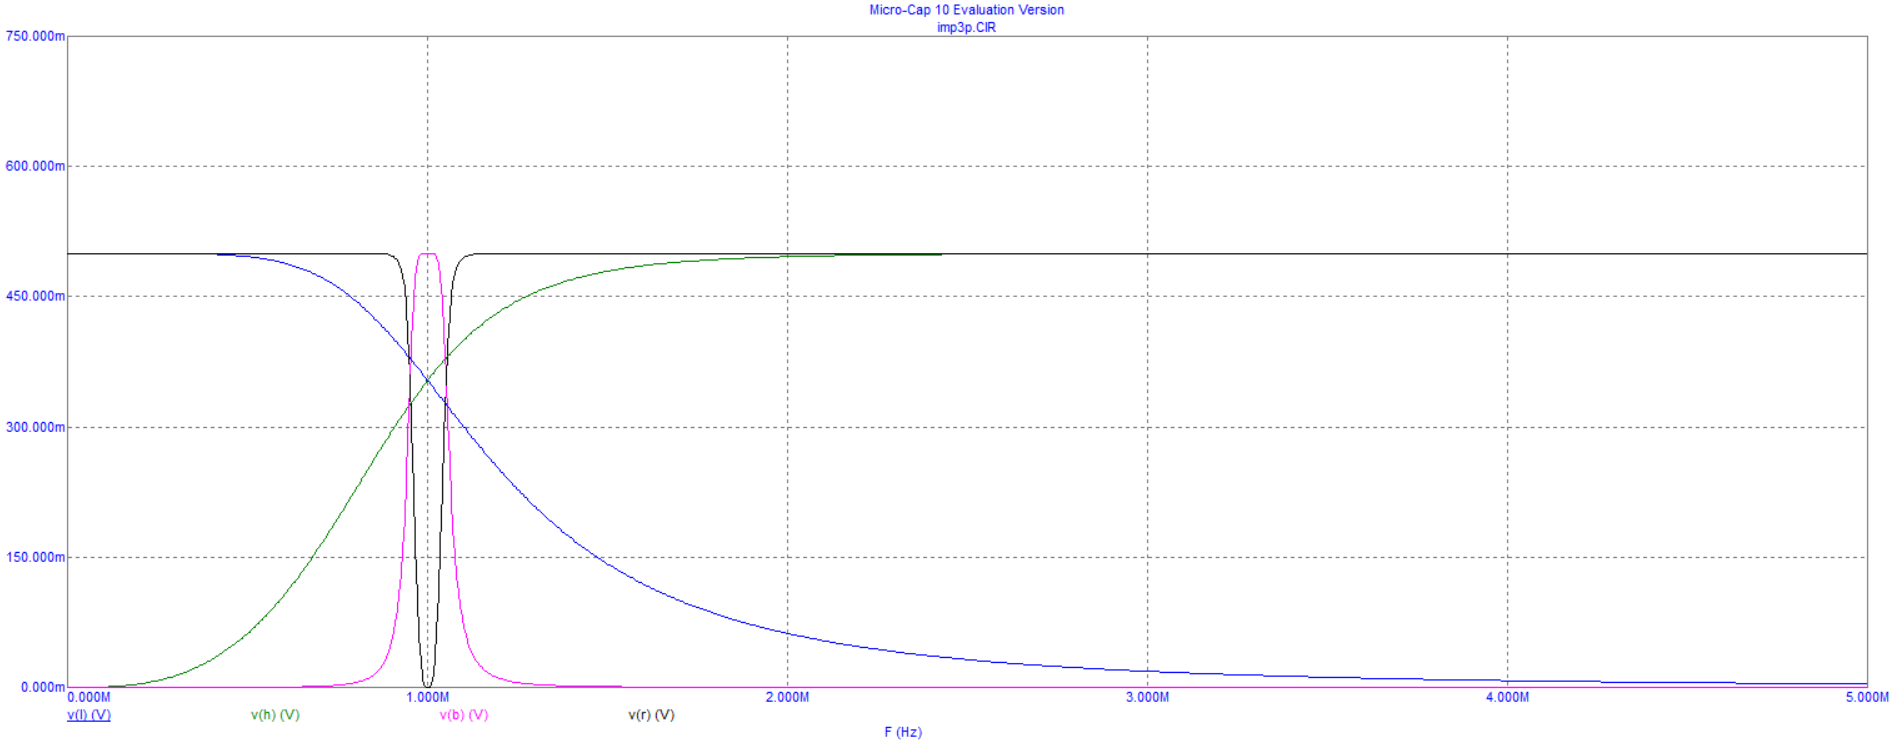
\includegraphics[width=1\textwidth]{част2.2.png}
	\label{fig:boiler}
\end{figure}

Сопоставим характеристики на едином графике.

\item Сравним частотные характеристики по напряжению и по мощности. Измерим уровни затухания по мощности на границах полос пропускания, там где затухание по напряжению составляет 0.7.

\textbf{У всех фильтров на этой частоте(1 МГц) затухание по мощности составляет 0.5}

Исследуем степень деградации характеристик фильтра нижних частот при варьировании сопротивления источника \textit{RSL} и нагрузки \textit{RLL} от 25 до 75 с шагом 25(на нулевой частоте).

\begin{center}
\begin{tabular}{|c|c|c|c|c|}
\hline 
 & \multicolumn{2}{c|}{RLL} & \multicolumn{2}{c|}{RSL} \\ 
\hline 
 & Напряжение & Мощность & Напряжение & Мощность \\ 
\hline 
25 & 0,33 & 0,44 & 0,66 & 1,77 \\ 
\hline 
50 & 0,5 & 1 & 0,5 & 1 \\ 
\hline 
75 & 0,6 & 1,43 & 0,4 & 0,625 \\ 
\hline 
\end{tabular} 
\end{center}

\item Изучим фазовые характеристики фильтров, измерим значения фазовых сдвигов на нулевой и бесконечной частотах:

\newpage

\begin{figure}[!h]
	\centering
	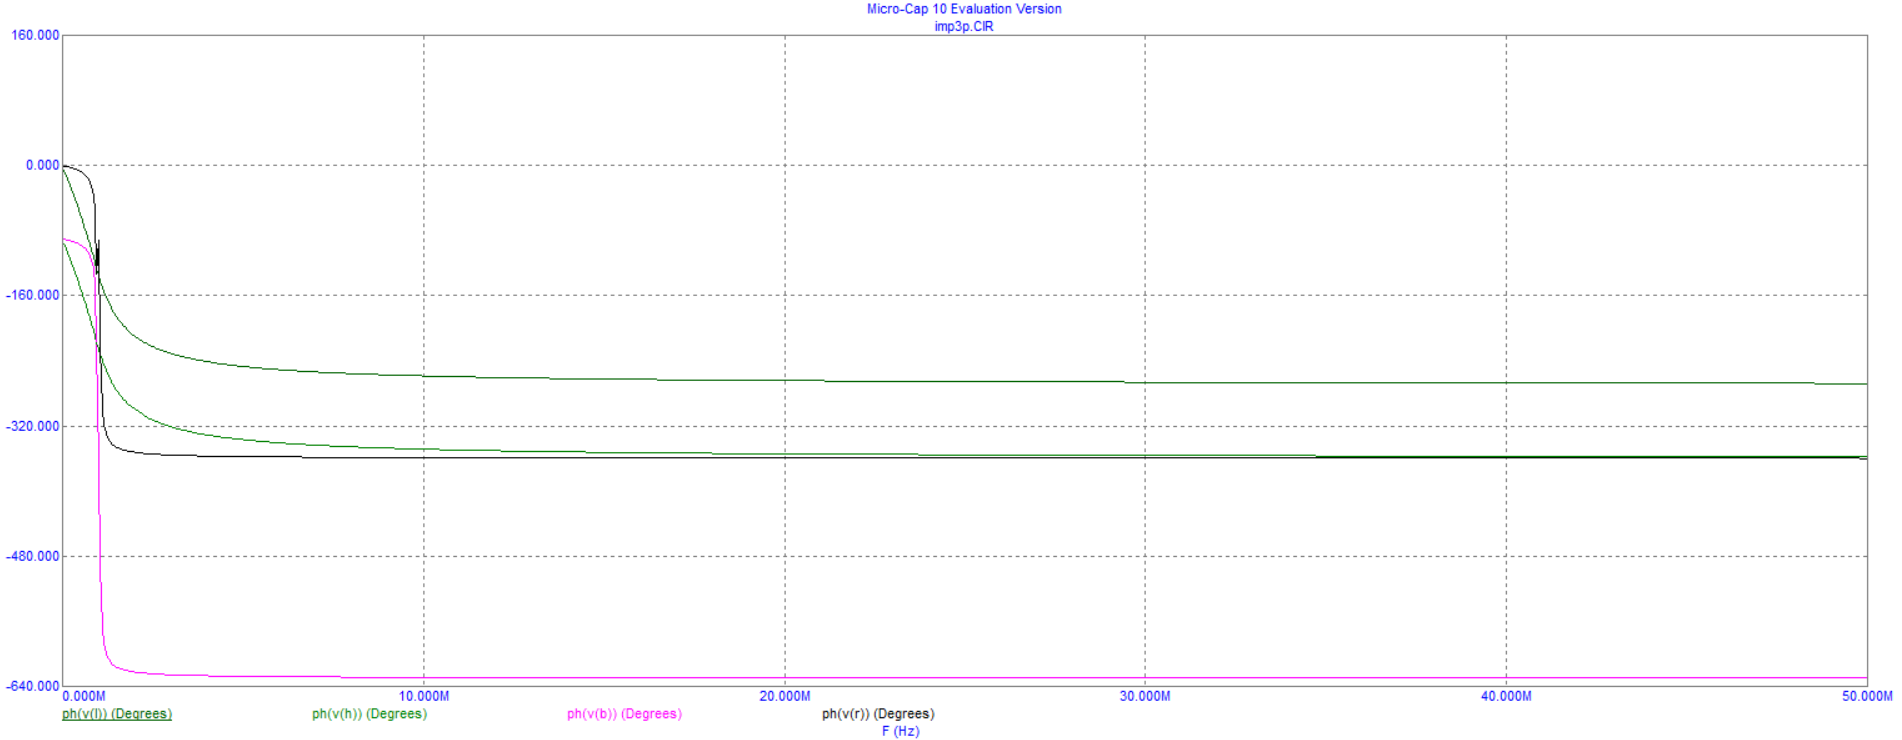
\includegraphics[width=1\textwidth]{2.4.png}
	\label{fig:boiler}
\end{figure}

\begin{center}
\begin{tabular}{|c|c|c|c|c|}
\hline 
$\omega$ & ФНЧ & ФВЧ & Полосовой & Режекторный \\ 
\hline 
0 & 0 & $-\pi/2$ & $3\pi/2$ & 0 \\ 
\hline 
$\infty$ & $-3\pi/2$ & $-2\pi$ & $-3\pi/2$ & 0 \\ 
\hline 
\end{tabular}
\end{center} 

\item Выведем логарифмическую частотную характеристику фильтра нижних частот в диапазоне $1Meg,100k$ (логарифмическая шкала) и измерим по ней уровни затухания в децибелах на частотах $0, f_0, 2f_0, 10f_0$:

\begin{center}
\begin{tabular}{|c|c|c|c|c|}
\hline 
$f$ & 0 & $f_0$ & $2f_0-$ & $10f_0$ \\ 
\hline 
$K(f_0)$ & -6 & -9 & -24,2 & -66 \\ 
\hline 
\end{tabular} 
\end{center}

\begin{figure}[!h]
	\centering
	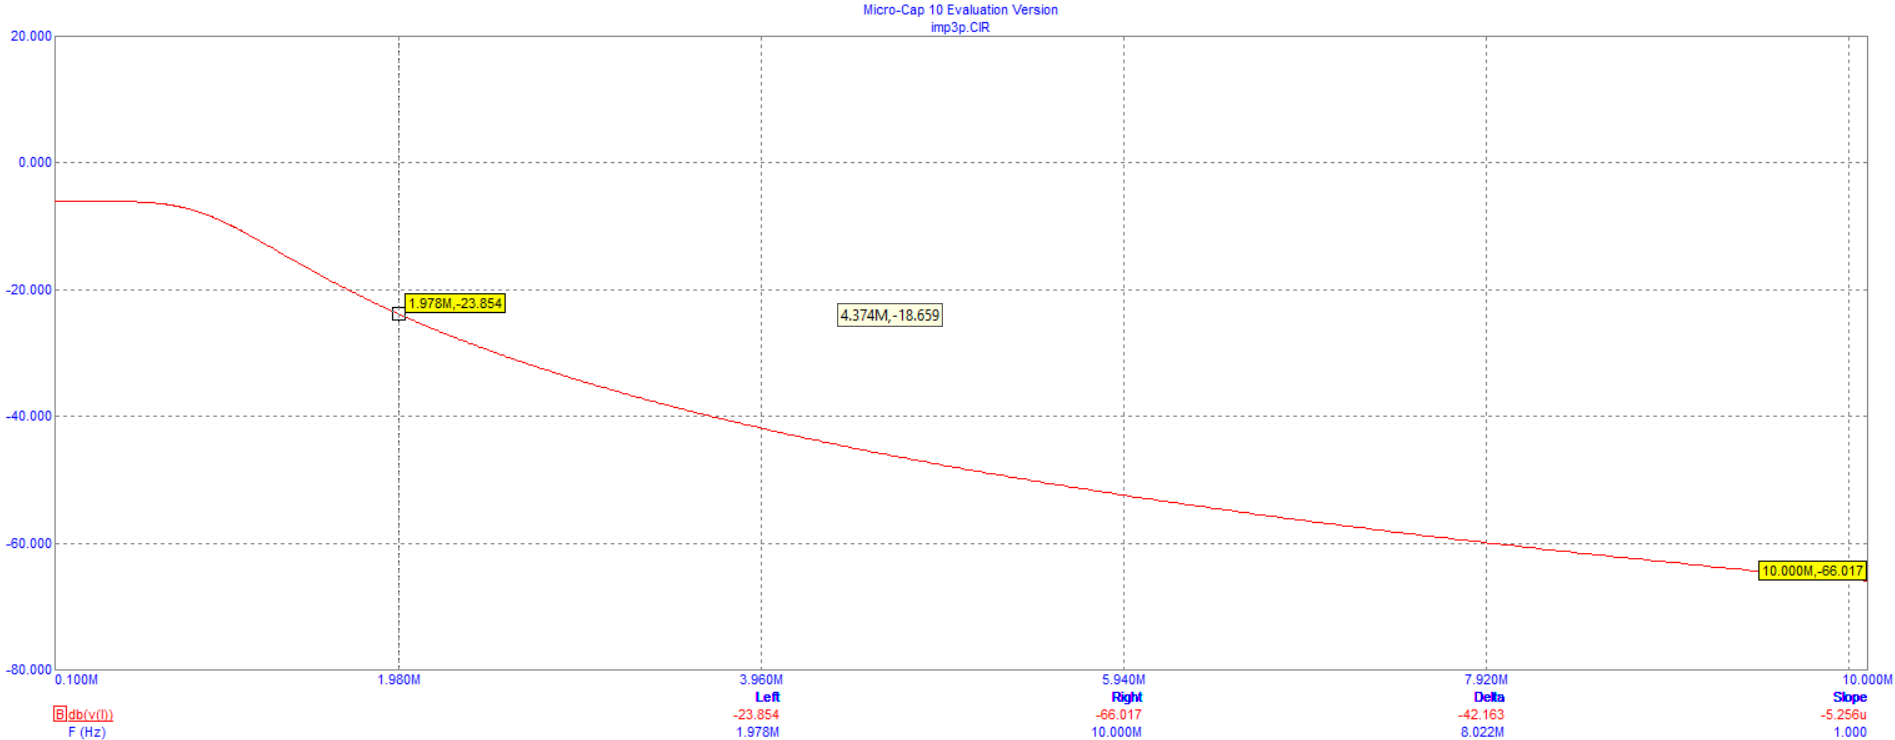
\includegraphics[width=1\textwidth]{2.5.png}
	\label{fig:boiler}
\end{figure}

\item Выведем логарифмическую частотную характеристику полосового фильтра в диапазоне $1500k,500k$ (линейная шкала) и измерим по ней уровень подавления на частоте $f_0$:

\[K(f_0) = -6 \: dB.\]

Измерим одностороннюю ширину $\bigtriangleup f$ полосы пропускания по уровню $-3 dB$ и уровень затухания при расстройках на $2\bigtriangleup f$, $10\bigtriangleup f$ от частоты $f_0$:

\[\bigtriangleup f = 48\: k\]

\[K(f_0 - 2\bigtriangleup f) = -25 \: dB, \quad K(f_0 + 2\bigtriangleup f) = -22 \: dB\]

\[K(f_0 - 10\bigtriangleup f) = -75 \: dB, \quad K(f_0 + 10\bigtriangleup f) = -60 \: dB\]

\item По логарифмической частотной характеристике режекторного фильтра в диапазоне частот $1500,500k$ измерим ширины полос по уровням $-3dB, -43dB, -63dB$:

\begin{center}
\begin{tabular}{|c|c|c|c|}
\hline 
$K(f_0 \pm \bigtriangleup f), \: dB$ & $-3$ & $-43$ & $-63$ \\ 
\hline 
$\bigtriangleup f$ & 50k & 10k & 4,5k \\ 
\hline 
\end{tabular} 
\end{center}

\begin{figure}[!h]
	\centering
	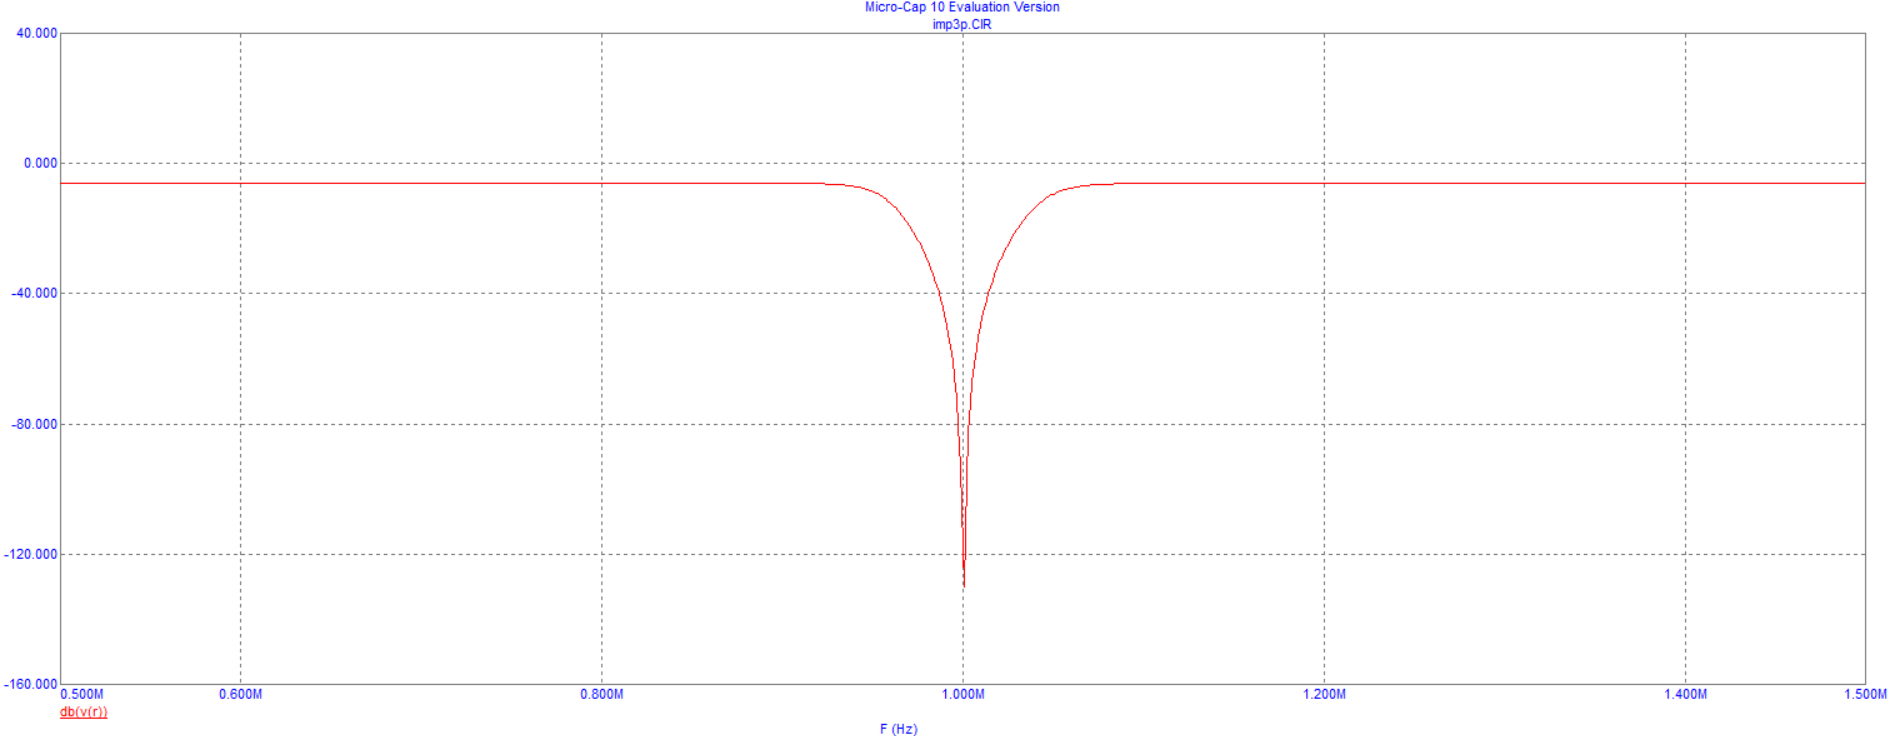
\includegraphics[width=1\textwidth]{2.7.png}
	\label{fig:boiler}
\end{figure}

\end{enumerate}

\subsection{Фильтры нижних частот высших порядков}

\begin{enumerate}

\item Откроем модель batt.cir, в которой реализованы фильтры Баттерворта нижних частот с параметрами $R_0 = 100, f_0 = 1MHz (L_0= 15.916, C_0 = 1.592n)$ порядков от 3 до 7. Изучим их частотные и переходные характеристики. По логарифмическим графикам в диапазоне $10Meg, 100k$ измерим затухания на частотах $f_0, 2f_0$ и $10f_0$:

\begin{center}
\begin{tabular}{|c|c|c|c|c|c|}
\hline 
Фильтр Баттерворта & n=3 & n=4 & n=5 & n=6 & n=7 \\ 
\hline 
$K(f_0), \: dB$ & -3 & -3 & -3 & -3 & -3 \\ 
\hline 
$K(2f_0), \: dB$ & -18 & -24 & -30 & -36 & -42 \\ 
\hline 
$K(10f_0), \: dB$ & -60 & -80 & -100 & -120 & -140 \\ 
\hline 
\end{tabular} 
\end{center}

\begin{figure}[!h]
	\centering
	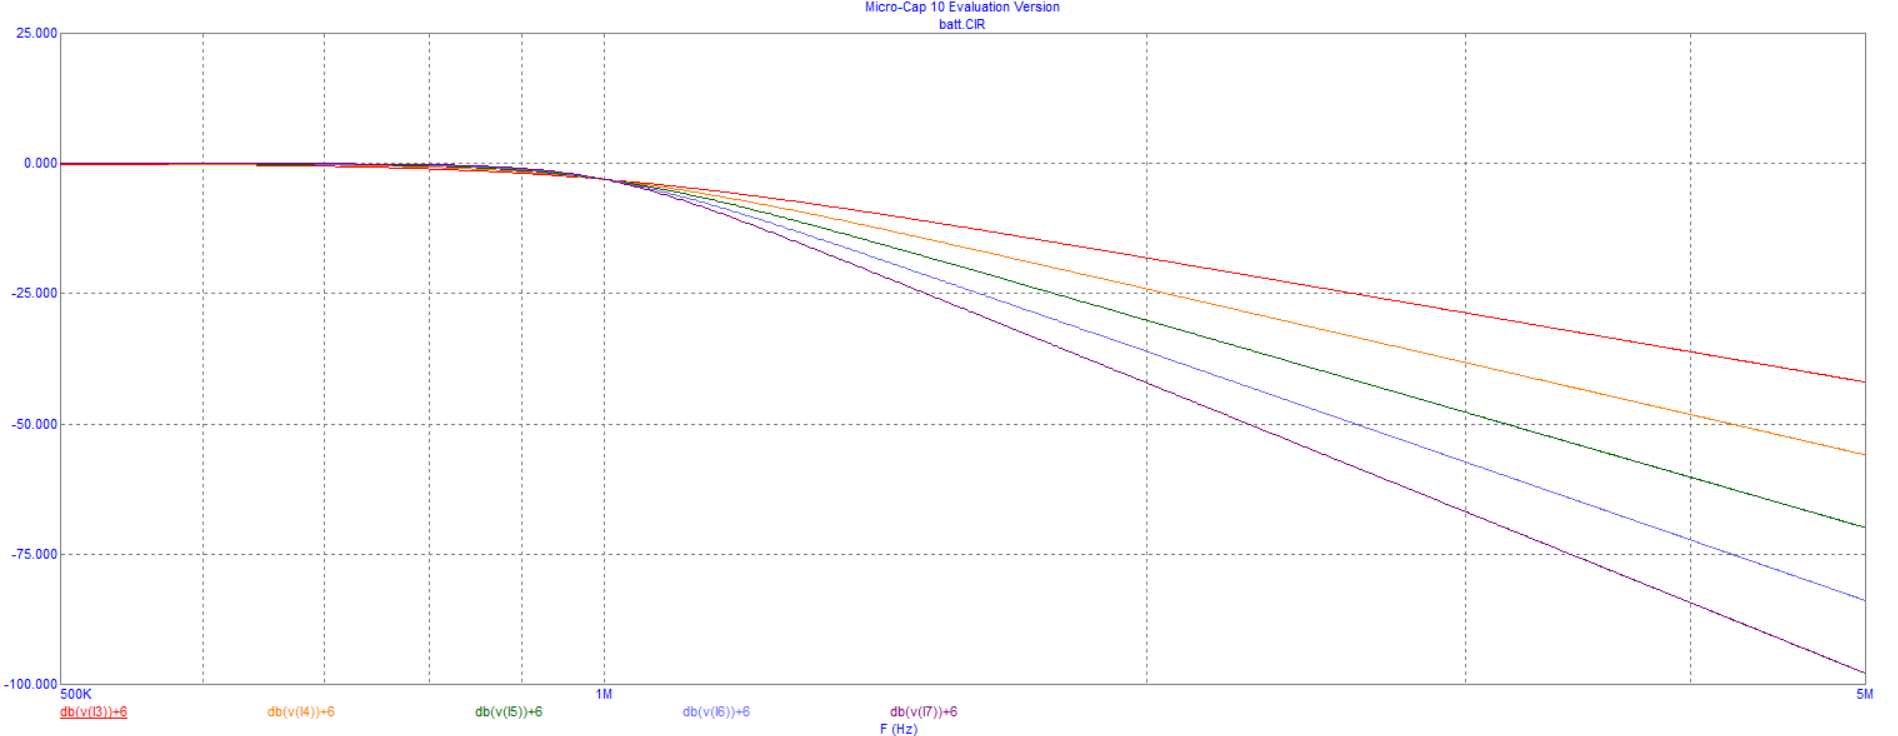
\includegraphics[width=1\textwidth]{3.1.png}
	\label{fig:boiler}
\end{figure}

\item Повторим те же исследования для фильтров Чебышева с неравномерностями 0.5 dB (файл cheb0-5.cir) и 3 dB (файл cheb3-0.cir)

\begin{center}
\begin{tabular}{|c|c|c|c|c|c|}
\hline 
$K(2f_0), \: dB$ & n=3 & n=4 & n=5 & n=6 & n=7 \\ 
\hline 
Баттерворта & -18 & -24 & -30 & -36 & -42 \\ 
\hline
Чебышева 0.5 dB & -19 & -31 & -42 & -54 & -65 \\ 
\hline
Чебышева 3.0 dB & -28 & -40 & -51 & -63 & -74 \\ 
\hline
\end{tabular} 
\end{center}

И  $10f_0$

\begin{center}
\begin{tabular}{|c|c|c|c|c|c|}
\hline 
$K(10f_0), \: dB$ & n=3 & n=4 & n=5 & n=6 & n=7 \\
\hline
Баттерворта & -60 & -80 & -100 & -120 & -140 \\ 
\hline 
Чебышева 0.5 dB & -63 & -89 & -115 & -141 & -167 \\ 
\hline 
Чебышева 3.0 dB & -72 & -98 & -124 & -150 & -176 \\ 
\hline 
\end{tabular} 
\end{center}

\end{enumerate}

\subsection{Фильтры пятого порядка}

\begin{enumerate}

\item 

\begin{figure}[!h]
	\centering
	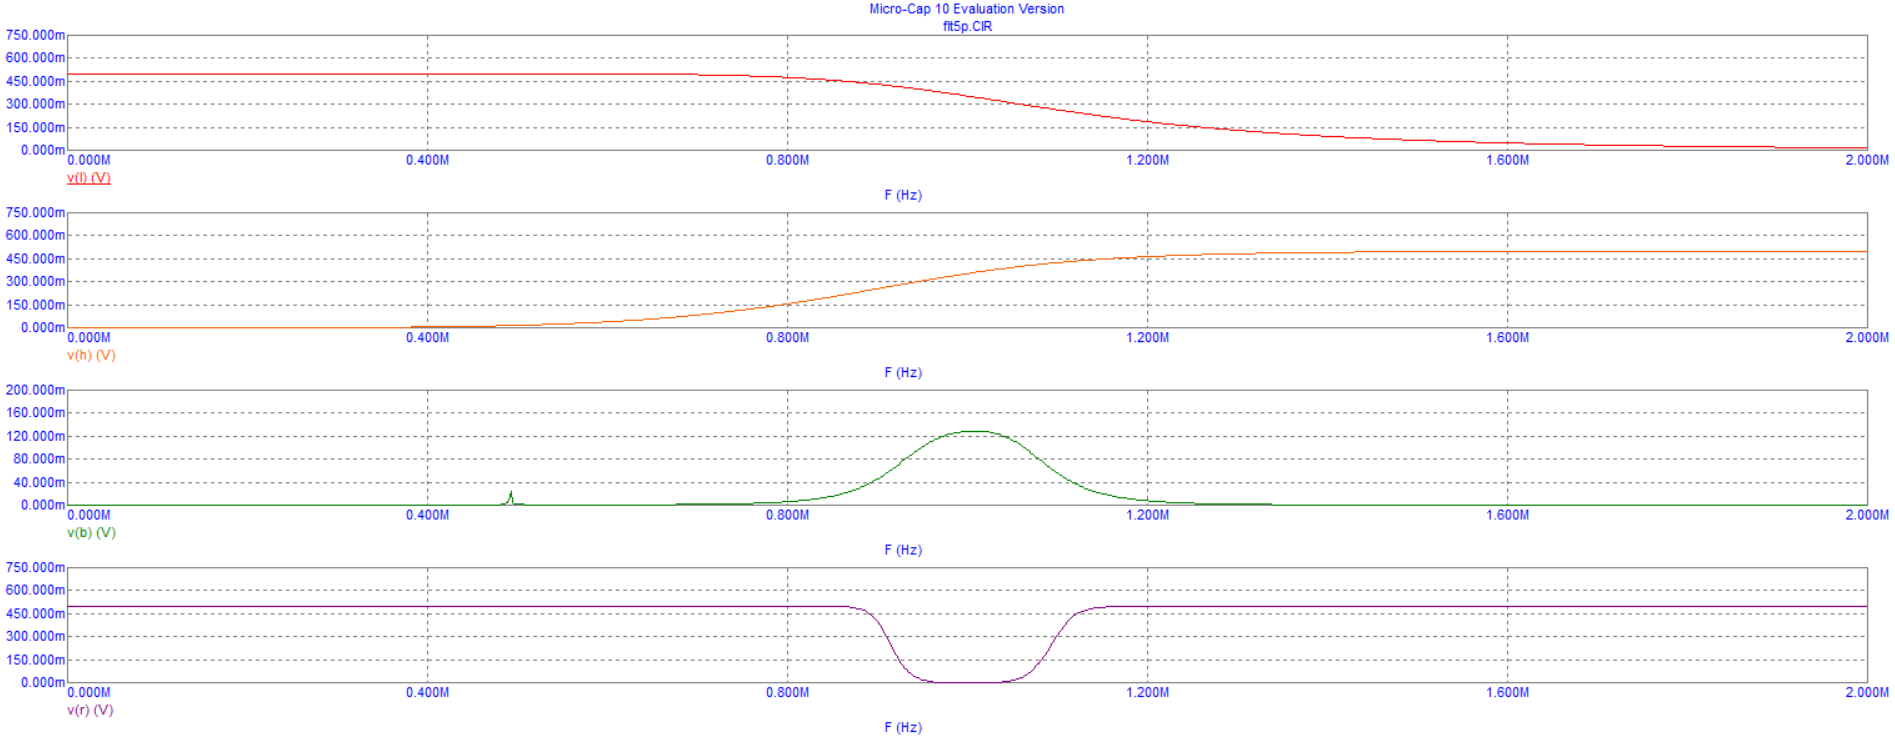
\includegraphics[width=1\textwidth]{4.2.png}
	\label{fig:boiler}
\end{figure}

Задам требуемые параметры и приведу частотные и переходные характеристики того, что получилось. Картинки приведу для фильтра Баттерворта.

\begin{figure}[!h]
	\centering
	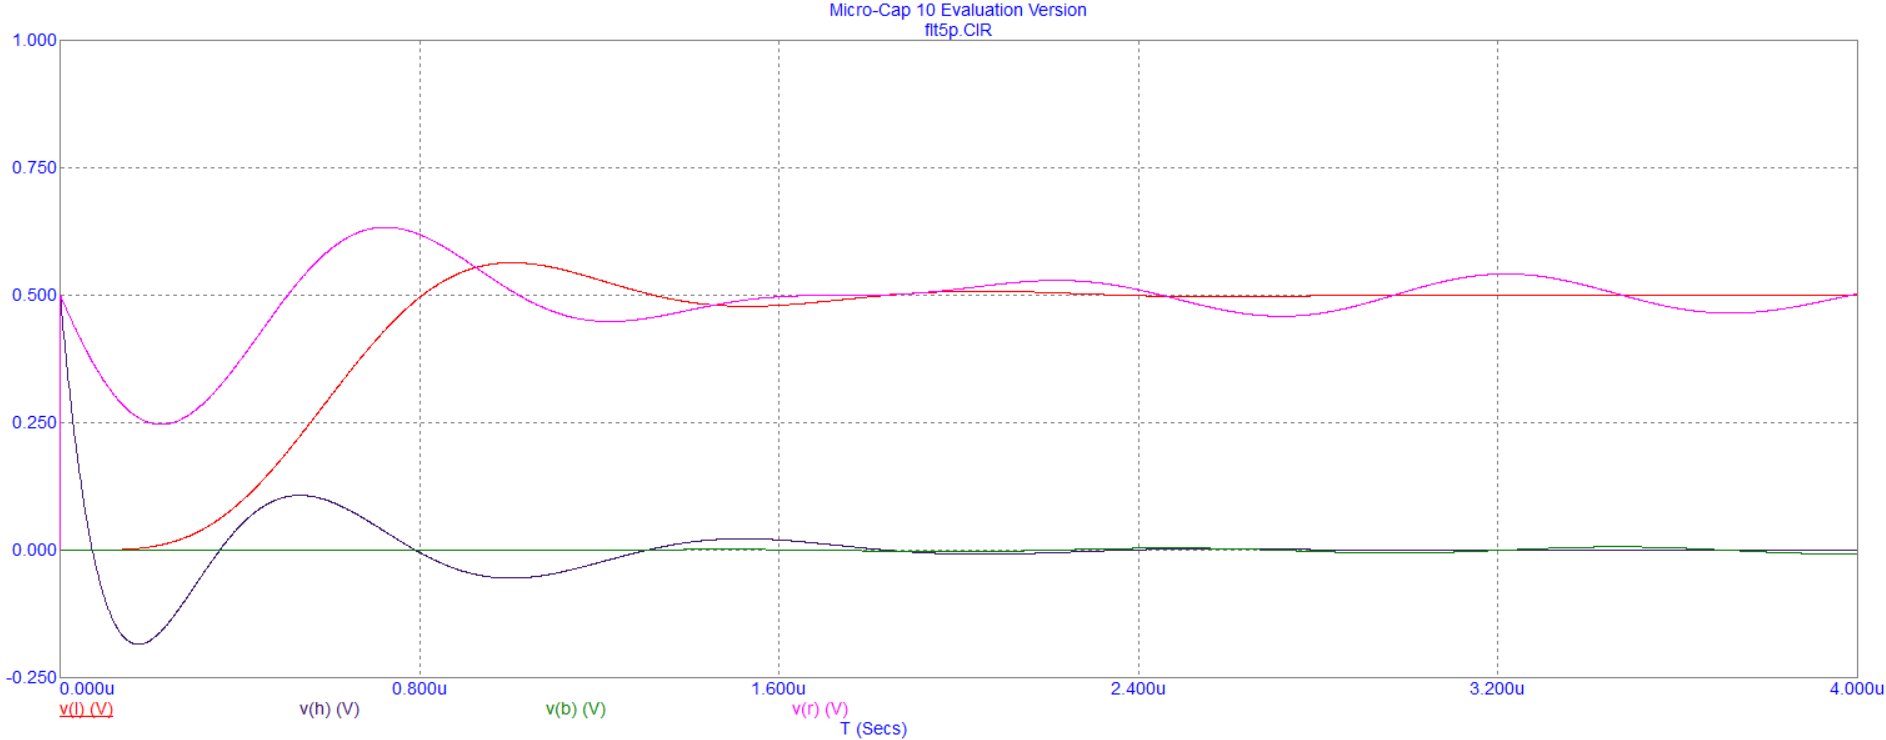
\includegraphics[width=1\textwidth]{4.3.png}
	\label{fig:boiler}
\end{figure}

Лучшие характеристики по затуханию фильтров этого порядка очевидны.

\end{enumerate}

\subsection{Семиполюсной фильтр}

\begin{enumerate}

\item Открыв файл \textit{pb7p.cir} реализуем семиполюсной фильтр Чебышева с неравномерностью 3 dB. для тракта усилителя промежуточной частоты приемника с параметрами $R_0 = 600$, $f_0 = 465 kHz$ и двухсторонней полосой $\bigtriangleup f = 24 kHz,$ $Q = \frac{f_0}{\bigtriangleup f} = 19.375$. По логарифмической частотной характеристике измерим избирательность по соседнему каналу - уровень затухания при расстройках на $\pm 24 kHz$ от $f_0$:

\begin{center}
\begin{tabular}{|c|c|}
\hline 
$+24 kHz$ & -72 dB \\ 
\hline 
$-24 kHz$ & -76 dB \\ 
\hline 
\end{tabular} 
\end{center}

Аналогично посчитаем разрешающую способность для фильтра Чебышева 0.5 dB:

\begin{center}
\begin{tabular}{|c|c|}
\hline 
$+24 kHz$ & -63 dB \\ 
\hline 
$-24 kHz$ & -67 dB \\ 
\hline 
\end{tabular} 
\end{center}

И для фильтра Баттерворта:

\begin{center}
\begin{tabular}{|c|c|}
\hline 
$+24 kHz$ & -41 dB \\ 
\hline 
$-24 kHz$ & -44 dB \\ 
\hline 
\end{tabular} 
\end{center}

\end{enumerate}


\section{Вывод}

Результаты моделирования, как и ожидается, тождественны теории. Все это позволяет сказать, что использованные методы расчета и анализа лестничных фильтров дают хорошие результаты в области применимости.


\end{problem}
\end{document}